\chapter{Implementation}
\section{DCE-MRI renography}
When the Contrast Agent is injected into the bloodstream, is starts its journey in the organism. It travels in the blood through the abdominal aorta, which branches  into the left and right renal arteries supplying the kidneys.  

Firstly, the CA reaches the renal cortex, where where a portion of it is filtered by the glomerulus from the blood to the Bowman's capsule in the process of glomerular filtration. Next, it is passed by the renal tubule to the renal medulla to finally be collected by the collecting system.   
Chemicals such as Gadolinium-based markers used in DCE-MRI that are freely filtered but neither reabsorbed nor secreted by the kidneys can be used for estimating the Glomerular Filtration Rate in quantitative DCE-MRI analysis.
\begin{comment}
This chapter describes in details the implemented method of the quantitative analysis of the kidney's function. Firstly, the subsequent steps of image processing and analysis are presented and the, the performance of the chosen PK models is compared. The aim is to chose the model, which would be the best for GFR estimation and to draw a conclusion if it can be considered a robust, reliable method for future applications. 
\end{comment}

This part of the thesis describes in details the implemented method of the quantitative analysis of the kidney's function from DCE-MRI. The chapter leads the reader through the subsequent steps of image processing and analysis to finally compare the performance of the chosen PK models. The aim is to choose the model, which allows obtaining the best results for GFR estimation on the give data and to draw a conclusion if it can be considered a robust, reliable method for future applications. 

\section{Materials and methods}
\subsection{DCE-MRI aquisition}
The dataset used in this project consists of forty DCE-MRI sequences. Each of the twenty healthy, non-smoking participants underwent two MRI examination at a~time interval of 7 days.
GdDOTA (Gadoteric Acid), which is a Gadolinium-based CA,  at a dose of 0.025\,mmol/kg was administrated as a bolus injection at 3\,ml/s in an antecubital vein followed by a 20 mL saline flush.
The examinations were performed on 32 channel 1.5 T whole-body scanner (Siemens Magnetom Avanto \cite{simens}) with a gradient strength\,=\,45\,mT/m and slew rate\,=\,200\,mT/m/ms using a~standard six-channel body matrix coil and table-mounted six-channel spine matrix coil for signal reception.
The 74 volumes, each consisting of 30 slices, covering the kidneys and the aorta were continuously acquired every 2.3 s for approximately 6 min in coronal-oblique plane.
The aquisition matrix was 192\,x\,192 whereas the voxel size was equal to 2.2\,x\,2.2\,x\,3\,mm$^3$
Th parameters of the used spoiled gradient recalled 3D FLASH pulse-sequence were echo time, $TE=0.8$\,ms, repetition time, $TR=2.36$\,ms, flip angle, $\alpha= 20^{\circ}$.

More information about aquisition of DCE-MRI data used in this project can be found in \cite{eikefjord2017dynamic}.
The few frames of the sample raw DCE-MRI sequence is shown in Figure~\ref{fig:set}.
\newpage


\begin{figure}[H]

\captionsetup[subfigure]{labelformat=empty,textformat=simple}
	\centering
	\subfloat[\textit{T} = 0\,Tp]{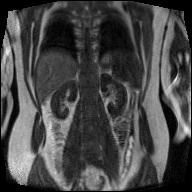
\includegraphics[height=0.24\linewidth]{img/preview/00}}\hspace{0.005\linewidth}
		\subfloat[\textit{T} = 9\,Tp]{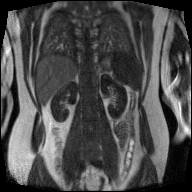
\includegraphics[height=0.24\linewidth]{img/preview/09}}\hspace{0.005\linewidth}
			\subfloat[\textit{T} = 12\,Tp]{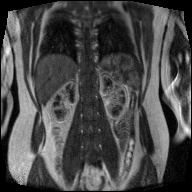
\includegraphics[height=0.24\linewidth]{img/preview/12}}\hspace{0.005\linewidth}
			\subfloat[\textit{T} = 16\,Tp]{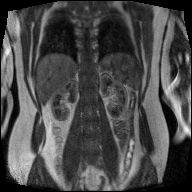
\includegraphics[height=0.24\linewidth]{img/preview/16}}\vspace{-4pt}
			
			\subfloat[\textit{T} = 18\,Tp]{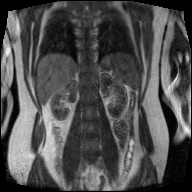
\includegraphics[height=0.24\linewidth]{img/preview/18}}\hspace{0.005\linewidth}
		\subfloat[\textit{T} = 22\,Tp]	{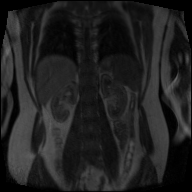
\includegraphics[height=0.24\linewidth]{img/preview/22}}\hspace{0.005\linewidth}
		\subfloat[\textit{T} = 26\,Tp]{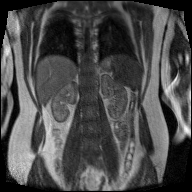
\includegraphics[height=0.24\linewidth]{img/preview/26}}\hspace{0.005\linewidth}
			\subfloat[\textit{T} = 30\,Tp]{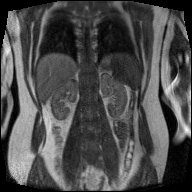
\includegraphics[height=0.24\linewidth]{img/preview/30}}\vspace{-4pt}

			\subfloat[\textit{T} = 34\,Tp]{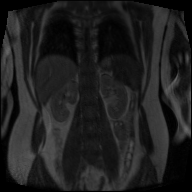
\includegraphics[height=0.24\linewidth]{img/preview/34}}\hspace{0.005\linewidth}
		\subfloat[\textit{T} = 39\,Tp]	{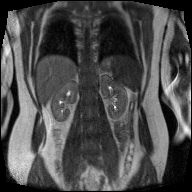
\includegraphics[height=0.24\linewidth]{img/preview/39}}\hspace{0.005\linewidth}
	\subfloat[\textit{T} = 55\,Tp]{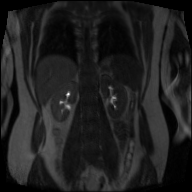
\includegraphics[height=0.24\linewidth]{img/preview/55}}\hspace{0.005\linewidth}
	\subfloat[\textit{T} = 73\, Tp]{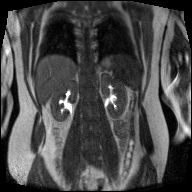
\includegraphics[height=0.24\linewidth]{img/preview/73}}
\vspace{0.5cm}
\caption[Sample DCE-MRI sequence of the healthy kidneys.]{Sample DCE-MRI of the healthy kidneys sequence. Tp is a given time point. Firstly the signal enhancement is observed in the renal cortex. Later, the tracer travels to the renal medulla and finally is collected by the collecting system.}
\label{fig:set}
\end{figure}


\subsection{GFR reference values}
Next to the DCE-MRI examinations, the participant had their GFR assessed by two commonly used in clinical practice chemical methods: the Serum-creatinine (SCr) blood test and iohexol-GFR tests. Creatinine is an endogenous indicator, which allows estimating GFR from validated algorithms.
Iohexol in terms is an exogenous marker which is used for accurate GFR measurement. The clinical characteristic of the participants is included in Table~\ref{tab:participants}

\begin{table}[h!]
\centering
\caption[Clinical characteristic of the participants]{Clinical characteristic of the participants. Taken from \cite{eikefjord2017dynamic}}
\label{tab:participants}
\begin{threeparttable}
\rowcolors{2}{}{beaublue!50}
\renewcommand{\arraystretch}{1.25}
\begin{tabular}{m{7cm} m{4cm}}
	\hline

 	Participants & 20\\
  	Gender (female/male) &16/4\\
  	Age (years) & 25 (20--38)\\
  	Height [m] & 1.71 $\pm$ 00.7\\
  	Weight [kg] & 66.2 $\pm$ 8.7\\
  	Body Mass Index (BMI) [kg/m\textsuperscript{2}] & 22.6 $\pm$ 2.1\\
  	Body Surface Area (BSA) [m\textsuperscript{2}]& 1.77 $\pm$ 0.14 (1.5--2.0) \\
  	Iohexol GFR [ml/min/m\textsuperscript{2}] &103 $\pm$ 10 (87--125)\\
  	SCr GFR [ml/min/m\textsuperscript{2}] & 110 $\pm$ 15 (81--128)\\
  \hline

\end{tabular}
\begin{tablenotes}%
\footnotesize{}%
\item Values in parentheses are ranges.
\item Plus minus values are means $\pm$ Standard Deviations (SD).
    \end{tablenotes}
	\end{threeparttable}
\end{table}

\subsection{Image processing and analysis}

\subsubsection{Motion correction}
One of the first fundamental problem encountered during DCE-MRI analysis is misalignment of 3D volumes across time slices. This misalignment of organs is a result of the patiens's respiratory motion as well as the heartbeat and bowel peristalsis and is unavoidable during examination. Studies have shown that even slight misalignment can lead to significant differences in intensity time-courses \cite{KidneySubsegmentation} and thus, motion correction of time series is essential for further analysis.

In order to remove 	the motion artifact, all files were motion-corrected across time points. For this purpose R programming language for statistical computing and graphics was used \cite{R} together with the package ANTsR \cite{ANTsR}, which provides quantification tools for biomedical images. 

As an initial step, for every time series, the algorithm extracted 3D volumes. Each extracted volume corresponded to data obtained in one time point. Next, the average image of the temporal volumes was calculated, which was a target image for image registration. Every temporal volume was then aligned to it and at the end they were combined back together into 4D time series.
As the misalignment concerns the inner structures, not the whole body and various organs have spatially variant geometric differences the modality of choice was the  \textit{Symmetric Normalisation} algorithm (SyN), which is the non-rigid deformable transformation utilizing \textit{Cross-correlation} (CC) as a similarity metric \cite{avants2011reproducible, avants2008symmetric, el2016current}. 

\subsubsection{Manual labelling}
In the next step, the labels of the whole left and right kidney were created. For this purpose, 3D volumes were extracted for every time frame and the slice with maximal signal enhancement of the kidneys was chosen (usually between 12--17 time slice). On this image, left and right kidney were manually delineated in coronal plane using ITK-Snap software \cite{itk-snap}. Additionally, few voxels of aorta (15--20) were labelled on maximal aortic enhancement time slice (9--10) . So obtained labels were then combined and propagated across the time points. The sample labels are shown in Figure~\ref{fig:labels}
All further analysis was implemented in Python programming language~v.~3.6 \cite{python}.

\begin{figure}
\captionsetup[subfloat]{captionskip=0.5cm}
	\centering
	\subfloat[Labels of the left and right kidneys ]{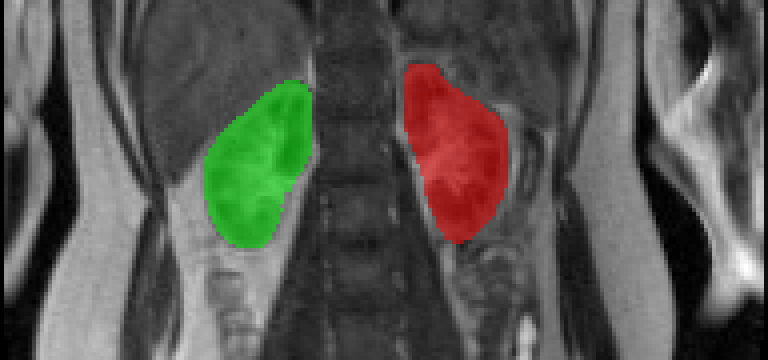
\includegraphics[width=0.48\textwidth ]{kidneys}}\hspace{0.02\textwidth}
	\subfloat[Label of aorta]{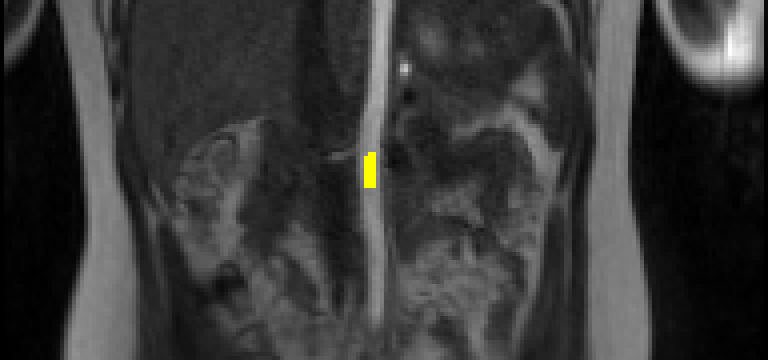
\includegraphics[width=0.48\textwidth]{aorta}}\\	
\vspace{0.5cm}
\caption[Sample labels of kidneys and aorta]{Sample labels of kidneys and aorta. Green and red are labels of the right and left kidney respectively, whereas yellow is the aorta label}
\label{fig:labels}
\end{figure}

\subsubsection{Pelvis removal}
Due to the fact that glomerular filtration takes place in renal renal parenchyma, pelvis had to be removed from the further analysis. 

Resulting from the physiology of the process, the three renal compartments (cortex, medulla, pelvis) can be distinguished from each other on the basis of their time courses, as shown in Figure~\ref{fig:timecourses}. Depending on the compartment, the rapid enhancement of the signal occurs in different period, which makes the shapes of the time intensity curves very unique.
From the \ref{fig:timecourses} it can be seen that the biggest variation is observed between pelvis and two other renal compartments.
Consequently, it can be separated by unsupervised clustering.
\vspace{0.5cm}

\begin{figure}[H]
	\centering
	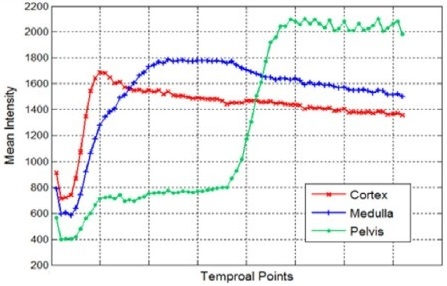
\includegraphics[width=11cm]{img/timecourses}
	\caption[Kidney compartments timecourses]{Kidney compartments timecourses \cite{KidneySubsegmentation}}
	\label{fig:timecourses}
\end{figure}

First of all, every of the the voxel belonging to the label of the kidney was described by the vector of seventy-four features as follows:
\begin{equation}
\label{eq:voxel}
\mathbf{v_{ijk}} = [S(0),\; S(1),\;...\;,\; S(72),\; S(73)],
\end{equation}
where $S(n)$ is the value of signal intensity in the time point $n$.

However, feature space of seventy-four dimensions is way too much for further analysis. High dimensionality of raw DCE-MRI data results in computational complexity, and thus memory and time consumption as well as numerical problems. What is more it contains a lot of noises \cite{KidneySubsegmentation}. To overcome this problems, the \textit{Principal Component Analysis} (PCA) \cite{pca} was applied.

PCA is a statistical procedure, which transforms the number of interrelated features into smaller set of uncorrelated variables. These so called \textit{Principal Components} (PCs) are a linear combination of the original variables \cite{dunteman1989principal}. As a result, after rotating the feature space, the first PC contains most variance, the last one the least and so on. In this way the dominant patterns are extracted while the noises are reduced~\cite{pca, jolliffe1986principal}. Further, every of the PC is characterised by a ratio of \textit{explained variance}, which indicates the portion of the dataset’s variance lying along the axis of each PC~\cite{handson}.

Applying the theory to practice, each voxel belonging to the kidney, initially described by forty-four features was described by a number of PCs:
\begin{equation}
\label{eq:voxelpca}
\mathbf{v_{ijk}} = [PC1,\; PC2,\;...\;,\; PCn]  
\end{equation}
The amount of PCs, $n$, was chosen as a minimum number of dimensions required to preserve 95\% of the data's total variance so that that the sum of the explained variances of  $n$ PCs was equal to at least 0.95 (usually between 4--6 PCs). The visual representation of the feature space with first three dimensions (PCs) for sample kidney is shown in Figure~\ref{fig:pca_plot}. Note that for better understanding, the clusters were already marked with different colors. 

\begin{figure}[H]
		\centering
		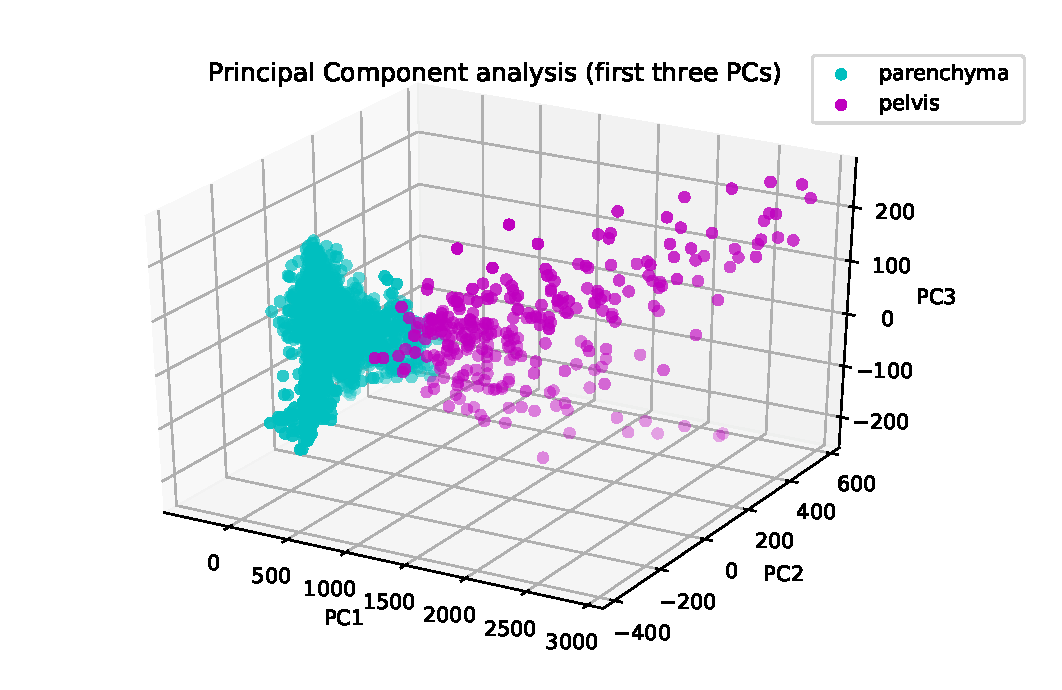
\includegraphics [height = 10cm]{pca}
		\caption [Principal Component Analysis for sample kidney]{Principal Component Analysis for sample kidney. The values in brackets are the ratios of explained variance for the given PCs. Note that the number of PCs was reduced to three for visualisation purpose}
		\label{fig:pca_plot}
	\end{figure}

To the dimensionally reduced data, the \textit{k-means clustering}} was applied in order to separate voxels into two groups: pelvis and renal parenchyma. 
The k-means is an unsupervised clustering algorithm aiming to divide the data into groups so that the diversity between the groups is maximised whereas the similarity within the single group is maximised  \cite{kmeans}. 

Given a data set $X=\{ \vec{x_1}...\vec{x_n}$\} in $m$-dimensional space (what actually corresponds to the $m$ features of a sample) the algoritm's objective is to minimize the square error function given by  \cite{kmeans, alsabti1997efficient}:

\begin{equation}
	\label{eq:kmeans}
	J = \sum_{j=1}^{k}\sum_{x_i \in S_j}(||x_i-c_j||)^2,
\end{equation}
where $||x_i-c_j||$ is  the Euclidean distance between a data point $x_i$ and the cluster centre $c_j$ of cluster $S_j$ from $k$ predefined clusters. It is achieved by the steps summarised in Algorithm~\ref{alg:kmeans}.

\vspace{16pt}
\begin{algorithm}[H]
\footnotesize
    \SetKwInOut{Input}{Input}
    \SetKwInOut{Output}{Output}
    \SetKwFunction{RandomlyChooseCentroids}{RandomlyChooseCentroids}
    \SetKwFunction{CalculateMeanOfPointsInCluster}{CalculateMeanOfPointsInCluster}
    \SetKwData{Centroids}{$(\vec{c_1}...\vec{c_k})$}
    \SetKwFunction{argminDistance}{argminDistance}
    
	\Input{number of clusters $k$,\\ set of points in $m$-dimensional space: $X=\{ \vec{x_1}...\vec{x_n}$\}}
	
    \Output{set of cluster labels of $X$: $L = \{l(\vec{x_i})\;i \in\{1...n\}\}$ ,\\ coordinates of cluster centroids: \Centroids}
    
    \BlankLine
    \BlankLine
    
    
	\DontPrintSemicolon
	\Centroids $\leftarrow$ \RandomlyChooseCentroids{$k$, $X$} \Centroids$\in X$\;
    
	\Repeat{none of \Centroids changes}{
\tcc {assign each data point to the closest centroid on the basis of Euclidean distance}
$l(\vec{x_i})\leftarrow$\argminDistance($\vec{x_i}$, $\vec{c_j}$) $j \in\{1...k\}$ \\
\Centroids$\leftarrow$  \CalculateMeanOfPointsInCluster{}  \tcc*{recalculate centroids} 
}
	\Return{$L$ , \Centroids} \tcc*{points divided into clusters} 
    
    
    \SetAlgoCaptionSeparator{.}
    \caption{K-means clustering}
    \label{alg:kmeans}
\end{algorithm}

\vspace{16pt}
To segment the kidney, the k-means algorithm was initiated with two clusters, $k$~=~2 and performed for points (kidney voxels) in ten-dimensional space (10 PCs).

Furter, for each of the identified clusters, the average time point, $T_{max}$ in which signal intensity reaches its maximum was calculated. 
Following the assumption that $T_{max\_pelvis}>T_{max\_parenchyma}$, the cluster with greater $T_{max}$ was marked as the pelvis and removed from the \textit{Region of Interest} (ROI).
The average time-intensity curves for two detected clusters in k-means clustering algorithm for sample kidney are presented in Figure~\ref{fig:clusters}. One can easily note the wash-in phase in pelvis takes place much later than in renal parenchyma. The results of the segmentation in turn are shown in Figure \ref{fig:segmentation}.  


\begin{figure}[H]
%\captionsetup[subfloat]{captionskip=0.5cm}
	\centering
	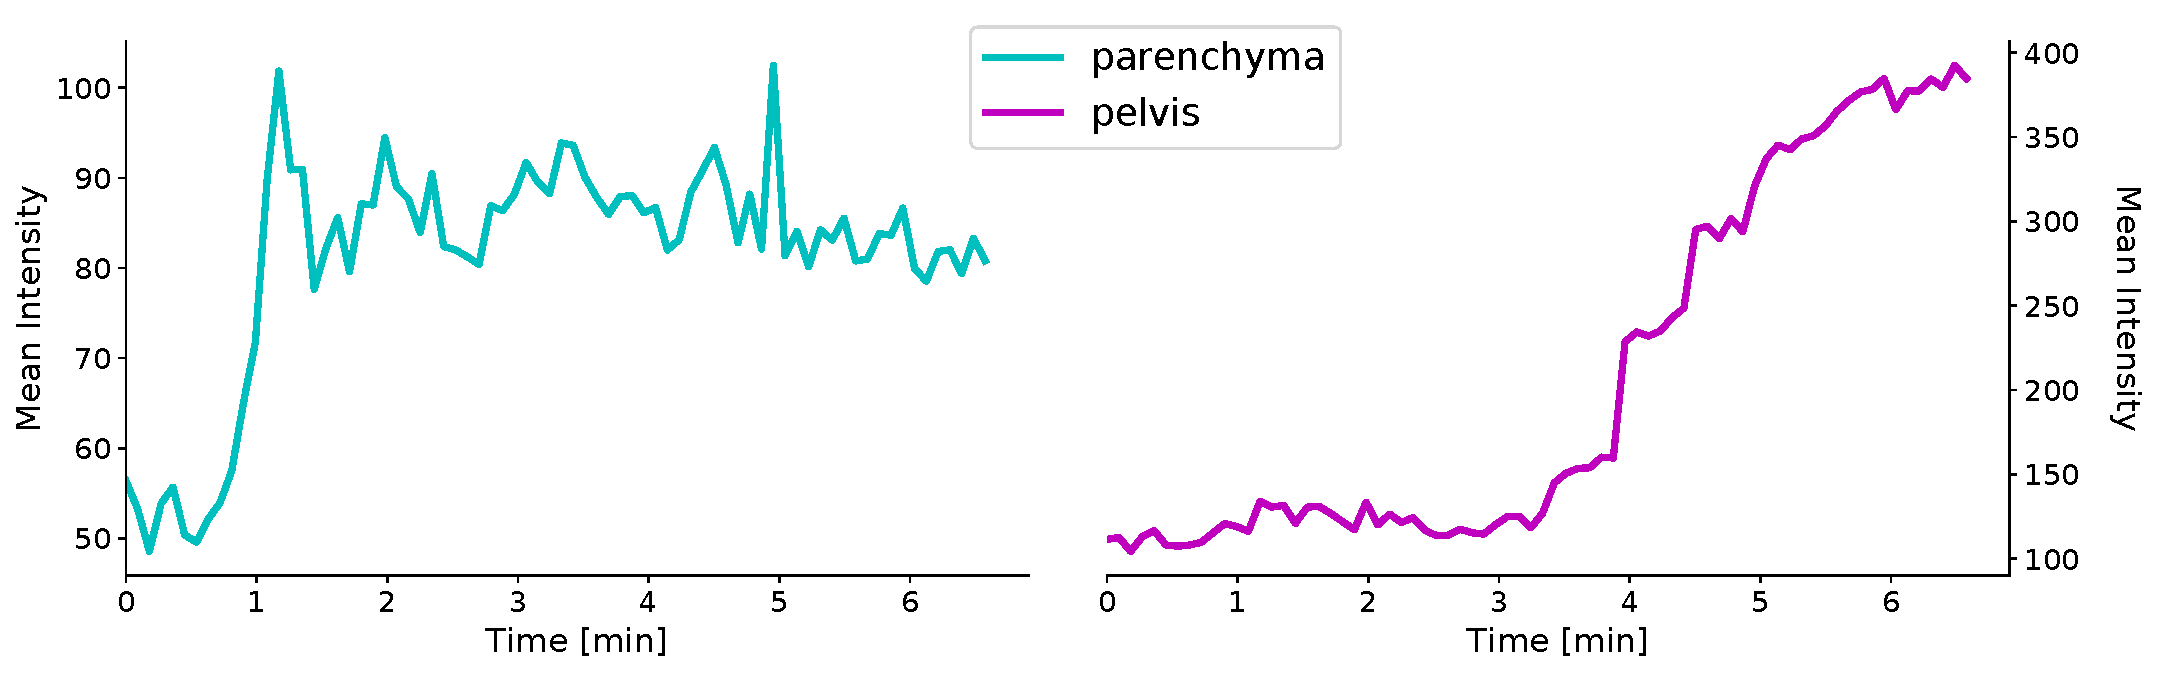
\includegraphics[width = \textwidth]{clusters}
	
\caption[Average time courses for two clusters detected in k-means algorithm]{Average time courses for two clusters detected in k-means algorithm performed for sample kidney}
\label{fig:clusters}
\end{figure}

\begin{figure}[H]
\captionsetup[subfloat]{captionskip=0.5cm}
	\centering
	\subfloat[Kidney segmentation]{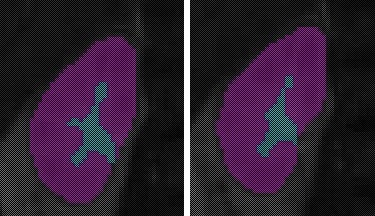
\includegraphics[width=0.48\textwidth ]{kidney_pelvis}}\hspace{0.02\textwidth}
	\subfloat[Renal parenchyma]{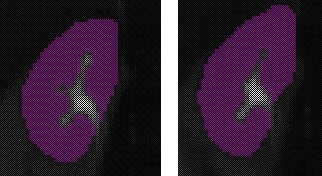
\includegraphics[width=0.48\textwidth]{no_pelvis}}\\	
\vspace{0.5cm}
\caption[Sample kidney segmentation with k-means clustering]{The results of the segmentation obtained with k-means clustering. Figure (a) shows two regions of sample kidney: the pelvis (cyan) and the renal parenchyma (magenta); Figure (b) presents the kidney after pelvis removal. The images were intentionally presented at Time point $Tp$ = 73, when the enhancement of the pelvis is big, for better visualisation}
\label{fig:segmentation}
\end{figure}

\subsubsection{Concentration-time curves}
Having labelled the proper ROI, the time has come for the principal part of the analysis, namely pharmacokinetic modelling.
All PK models used during quantitative DCE-MRI analysis call for determining both the tissue, $C_t(t)$, and blood plasma, $C_p(t)$, concentration as a~function of time. In our case, the $C_t(t)$ is the mean concentration in renal parenchyma, whereas the
$C_p(t)$, can be derived from  AIF, which is a concentration in a blood vessel feeding the kidney (aorta).
Thus, they were calculated in the next steps of the project.  

For each of the kidney, as well as for the aorta, the mean intensities of the voxels included in the particular labels were calculated at the each time point and the intensity time courses were plotted. Sample time courses are shown in Figure~\ref{fig:temporal_points}.

\vspace{10pt}
\begin{figure}[H]
%\captionsetup[subfloat]{captionskip=0.5cm}
	\centering
	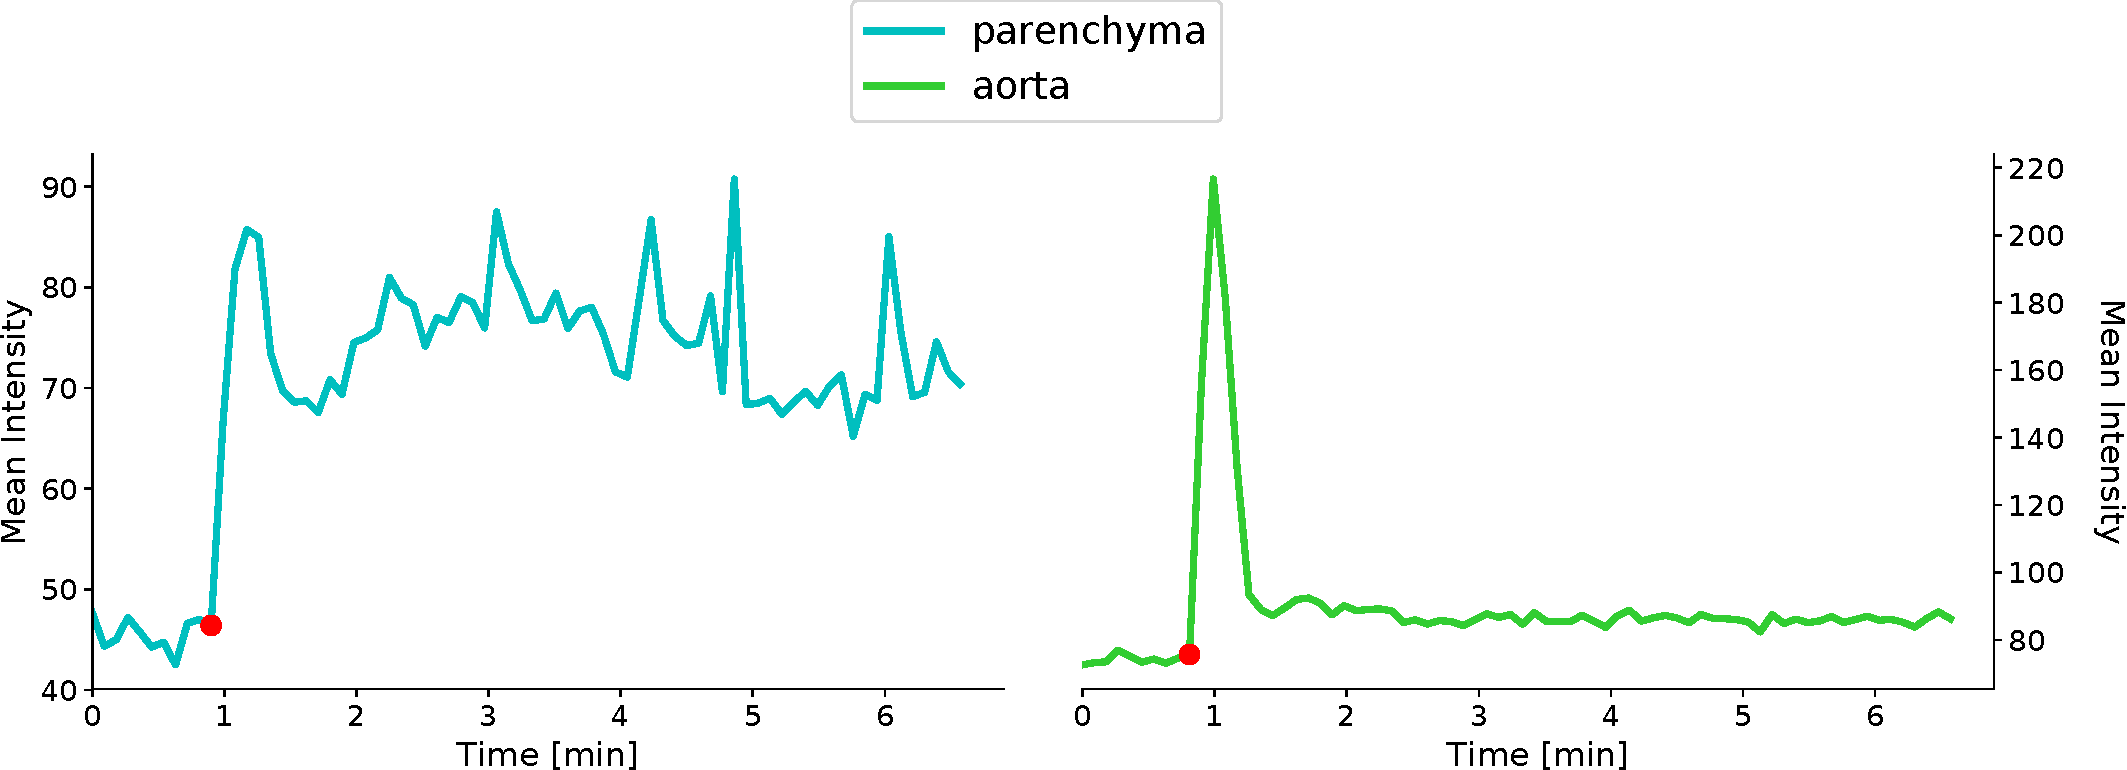
\includegraphics[width = \textwidth]{temporal_points}
	
\caption[Sample average time-intensity curves for a kidney and aorta with marked last points of the baseline]{Sample average time-intensity curves for a kidney and aorta. Red dot is $T_{baseline}$, the last point of the baseline}
\label{fig:temporal_points}
\end{figure}




Assuming the linear relation between tracer concentration and signal intensity $S(t)$ dictated by the low dose of Ga-based CA, the tracer concentration can be expressed as:
\begin{equation}
	\label{eq:conversion}
	C(t) = S(t)-S_0,
\end{equation}
where $S_0$ is the baseline signal, which is the average signal intensity among the time before the administration of CA. 
In order to determine $S_0$, the time point before rapid signal increase, $T_{baseline}$ had to be found  as marked with red dot in Figure \ref{fig:temporal_points}.

To achieve it, firstly, for the purposes of the examination of the function changes, the median filter  with the $kernel\;size = 5$ was applied in order to smooth the signal and eliminate artificial  peaks and valleys, as shown in Figure~\ref{fig:median}  
In next step, for every intensity time course under analysis, its derivative was calculated. The derivative describes the instantaneous rate of change of the function. It tells how fast the output of the function (signal intensity) changes compared to the independent variable (time) \cite{calculus} and seems to be a perfect solution to the problem, which comes down to the finding the most rapid signal change. 
Because of one's interests is detection only of the function's increases, not decreases, the points, in which the derivative is negative were neglected, $S'(t)<0\leftarrow0$. So modified derivative of the sample kidney and aorta are shown in Figure~\ref{fig:derivative}.

Now, all that had to be done to find $t_{baseline}$ was to find the point, in which the derivative of the signal intensity time course reaches its maximum, $t_{baseline}~=~argmax\;S'(t)$. Having it determined, the $S_0$ was calculated as the mean signal intensity value from the beginning of the measurement ($t=0$) to $t_{baseline}$. Finally, the CA concentration in the tissue and aorta were calculated according to the Formula~\ref{eq:conversion}. The results of intensity-concentration conversion for sample time curves are shown in Figure~\ref{fig:conversion}. 
\begin{figure}[H]
%\captionsetup[subfloat]{captionskip=0.5cm}
	\centering
	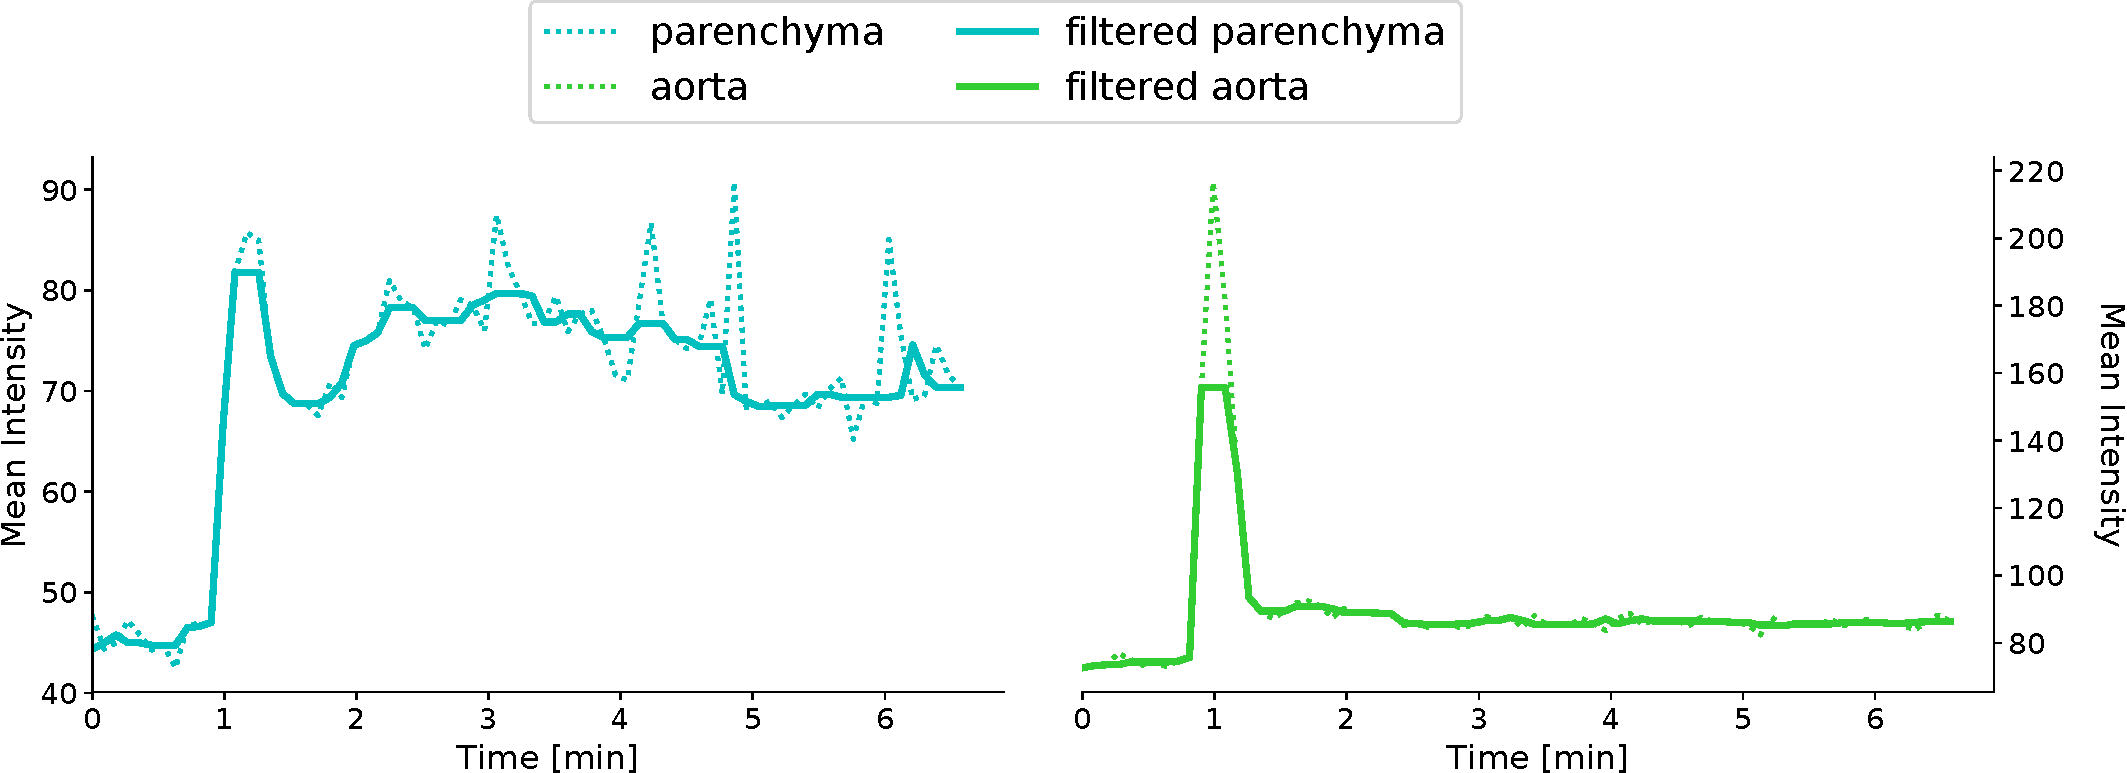
\includegraphics[width = \textwidth]{median2}
\caption[Sample average time-intensity curves for a kidney and aorta with applied median filter]{Sample average time-intensity curves for a kidney and aorta with applied median filter. Note that cut peak of the aorta's signal is a result of the median filter and is present only during baseline removal step}
\label{fig:median}
\end{figure}

\begin{figure}[H]
%\captionsetup[subfloat]{captionskip=0.5cm}
	\centering
	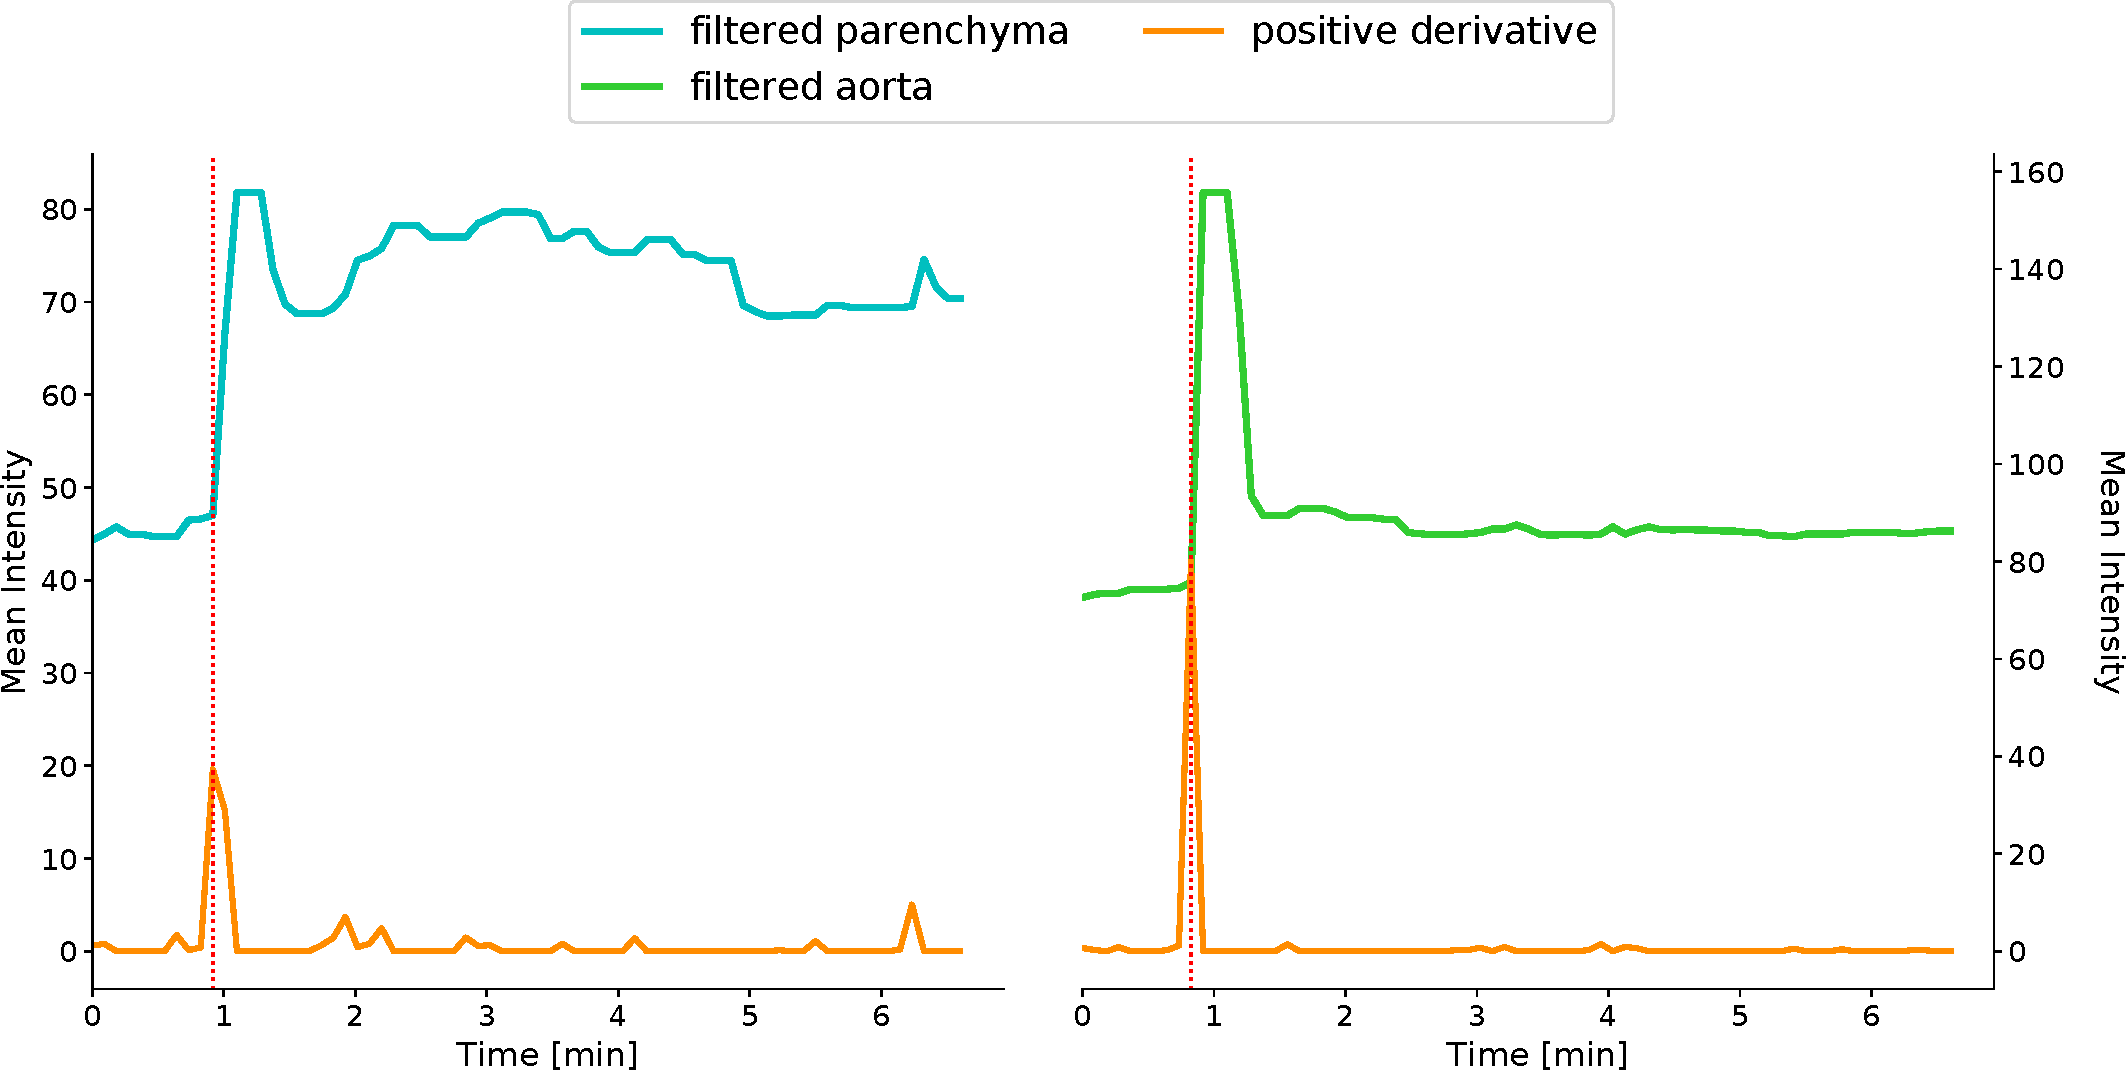
\includegraphics[width = \textwidth]{derivative}
\caption[Positive derivative of the sample kidney and aorta intensity time courses]{Positive derivative of a sample kidney and aorta intensity time courses. The horizontal line indicates the time point, in which the derivative reaches its maximal value}
\label{fig:derivative}
\end{figure}

\begin{figure}[H]
%\captionsetup[subfloat]{captionskip=0.5cm}
	\centering
	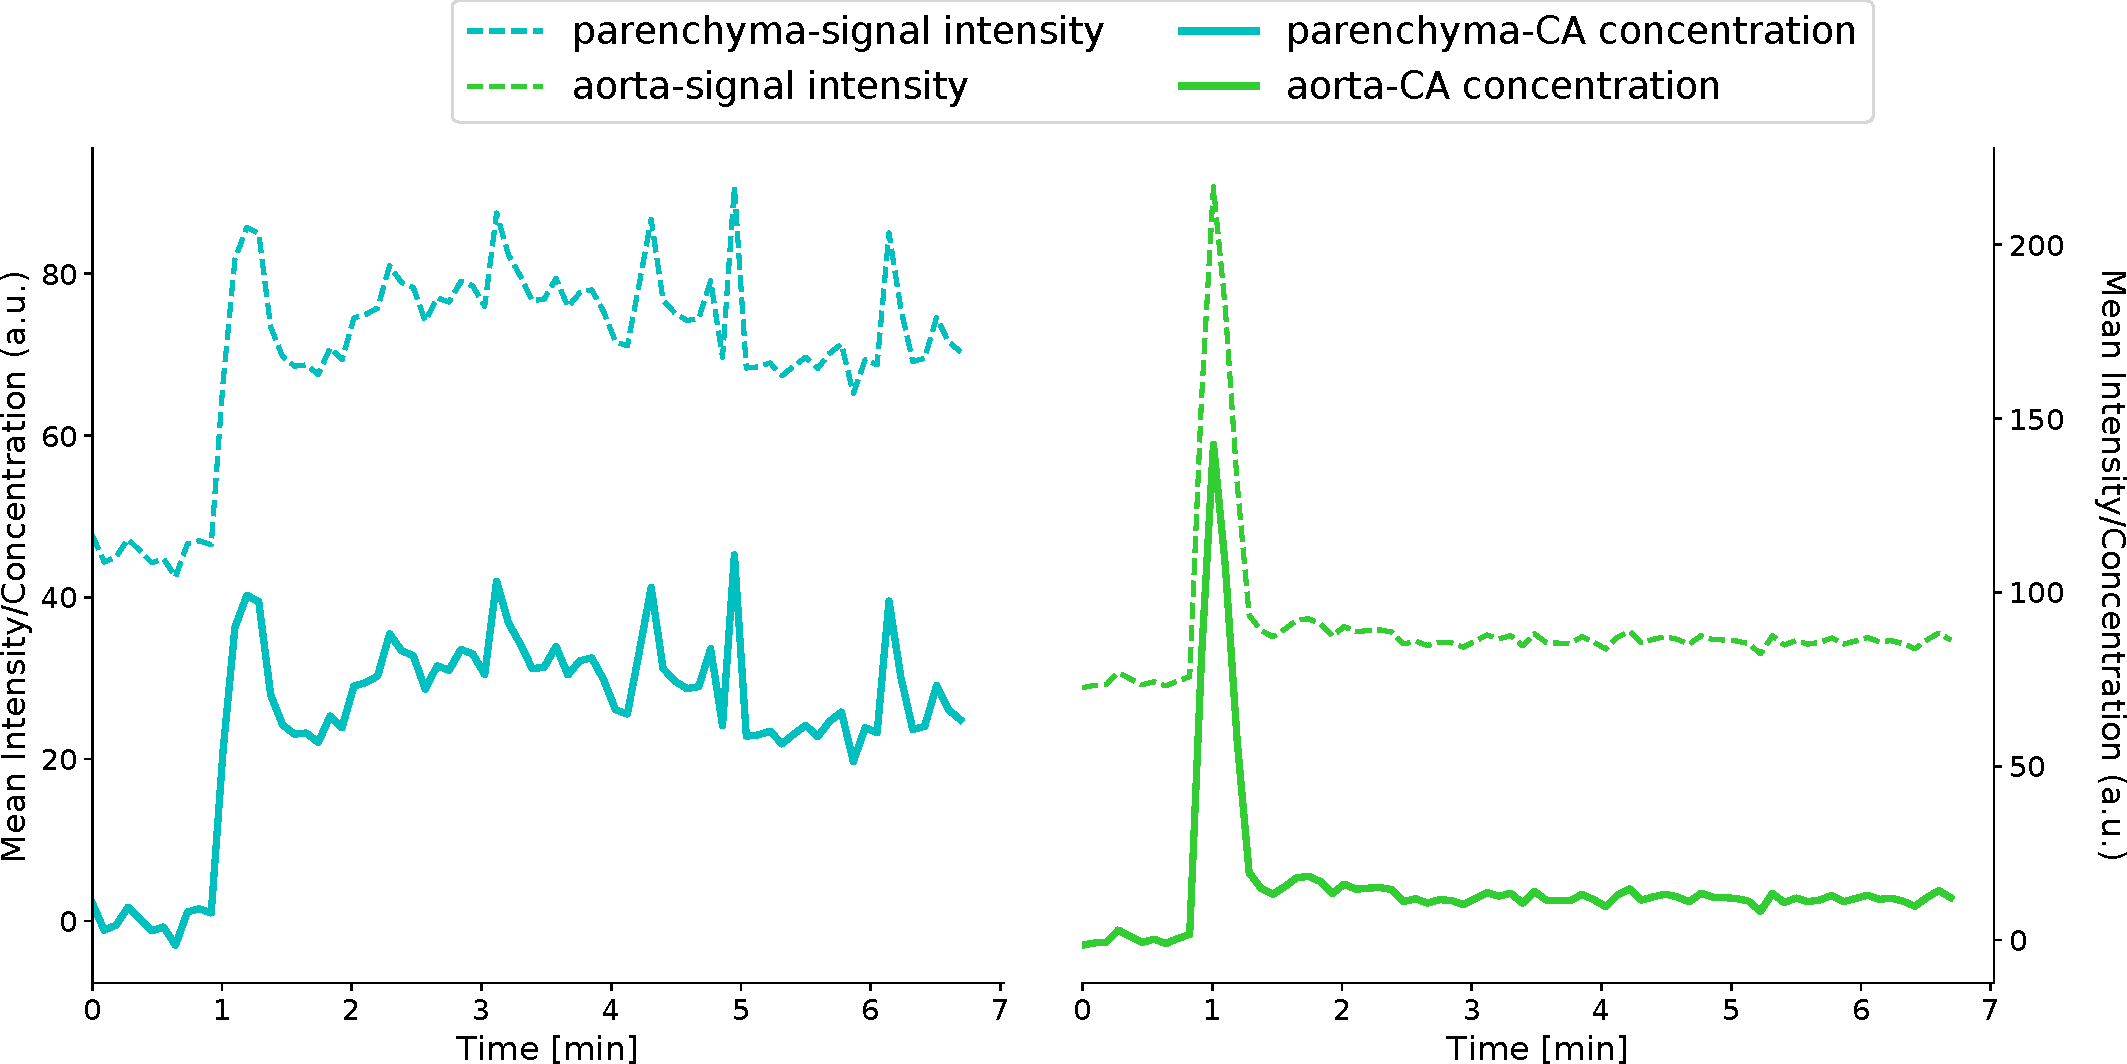
\includegraphics[width = \textwidth]{conversion}
\caption[Time courses of a sample kidney and aorta after intensity-concentration conversion]{Time-intensity curves of a sample kidney and aorta converted into concentration-time curves}
\label{fig:conversion}
\end{figure}


\subsubsection{Pharmacokinetic modelling}

Having determined the AIF and the concentration time course for the renal parenchyma, almost all components necessary for the renal  quantitative evaluation were obtained. Almost, but not all. One should take into consideration the fact that AIF is the concentration of CA in the blood of the aorta, which consist of both the red blood cells and the blood plasma. Gadolinium-based Contrast Agents, however, distribute in plasma rather than whole blood, so their effective plasma concentrations must be considered. Thus the \textit{Hematocrit} (Hct) correction were performed as follows \cite{tofts2010t1}:
\begin{equation}
	\label{eq:hematocrit}
	C_{p}(t) = C_{a}(t) / (1-Hct),
\end{equation}
where $C_p$ is plasma concentartion, $C_a$ is concentration in the aorta defined by AIF and $Hct$ is s the volume percentage of red blood cells in blood. In this study, the value was taken from the literature as an average population value and was equal to $Hct=0.42$ \cite{tofts2010t1}.

Finally, the long-awaited PK modelling could have been performed. The models of choice were the Toft's model, Extended Toft's model, Patlak model and 2-Compartment Exchange model. 
 
\paragraph{Toft's model}
\begin{comment}
The assumption underlying the TM is that the eect of vascular tracer can be ignored,
i.e. that the vascular signal is small in comparison to the tissue signal. For this
purpose the modelling of the tracer transport through an extracellular extravascular
compartment (with fractional volume ve) suces. When considering a simple diusion
mechanism active transport processes and dierences in viscosity or pressure can be
neglected. In this case the transport of indicator Ktrans into and out of the EES is
assumed to be the same in both directions. For such a one-compartment system the
mass balance equation is known from the previous section:
with a negligible
amount of intravascular trace
\end{comment}

\textit{The Tofts model} \cite{tofts1991measurement} (TM) assumes the diffusion of the tracer from the blood plasma at rate specified by the transfer constant $K_{trans}$ $(min^{-1})$ and its return at the rate $k_{ep} = K_{trans}/v_e$ $(min^{-1})$. This model assumes that the amount of intravascular tracer is negligible comparing to the tissue signal. This assumption leads to: $C_t(t) = v_eC_e(t)$. According to the Tofts model, the tissue concentration is specified by the formula \cite{tofts2010t1, tofts1991measurement}:
 
\begin{equation}
	\label{eq:toft}
	\frac{dC_{t}(t)}{dt} = K_{trans}(C_p(t)-C_t(t)/v_e)
\end{equation} 
The solution obtained according to the procedure presented in Chapter~\ref{chapter:pk} is:
\begin{equation}
	\label{eq:toft2}
	C_{t}(t) =C_p\circledast K_{trans}e^{-k_{ep}t} =K_{trans}\int_{0}^{t}C_p(t')e^{-k_{ep}(t-\tau)}d\tau  
\end{equation}

\paragraph{Extended Toft's model}
While the Toft's model neglects intravascular contribution assuming weak vascularization of the tissue, the Extended Toft's model \ref{tofts1997modeling} does take it into account. The tissue concentration is described by the formula:
\begin{align}
	\label{eq:extended_toft}
	\nonumber C_{t}(t) &= v_pC_p(t)+\\ 
	&+ K_{trans}\int_{0}^{t}C_p(t')e^{-(K_{trans}/v_e)(t-t')}dt', 
\end{align}
where $v_p$ is the fractional plasma volume. 

In Toft's and extended Toft's models the free parameters $K_{trans}$, $v_e$ and $v_p$ are estimated by fitting the model to obtained in DCE-MRI examinations time concentration curves.  

\paragraph{Patlak plot}
Another proposed approach is the graphical one called Patlak plot \cite{patlak1983graphical}. Patlak plot neglects $k_{ep}$ due to the low permeability and short examination time. As a result tissue concentration is expressed as:

\begin{equation}
	\label{eq:patlak}
	C_{t}(t) =v_pC_p(t) + K_{trans}\int_{0}^{t}C_p(t')dt'  
\end{equation}
The above equation is the linearised as:
\begin{equation}
	\label{eq:patlak_lin}
	Y = K_{trans}X +v_p,  
\end{equation}
where $Y=C_t(t)/C_p(t)$ and $X=\int_{0}^{t}C_p(t')dt'/C_p(t)$. The free parameters $K_{trans}$ an $v_p$ can be then estimating by constructing a linear plot and calculating its slope and intercept respectively.


\subsubsection{GFR estimation}

\section{Results}



\begin{comment}



 
\subsection{Manual labelling of kidneys and aorta} 
\label{subsec:labelling}
  
 


\newpage
\subsection{Pharmacokinetic modelling}
The time-dependent distribution and disposition of a substance in a living system can be described by phamacokinetic (PK) models~\cite{gerlowski1983physiologically}. They aim to characterise a physiologic system by decomposing them into interacting compartments. Every of them is a homogenous, well-mixed space with the uniform tracer distribution \cite{PMID:20540902}.




PK models have very wide clinical application: from estimating the optimal drug dose to determining safe working environment while working with toxins  \cite{gerlowski1983physiologically}.
Given the fact that the contrast agent used in DCE-MRI examination can be considered as a substance flowing through the organism, pharmacokintetic modelling can also be used in analysis of so obtained data.   
This approach, called the parametric one, is based on fitting mathematical model to acquired tissue concentration time courses. In this way, the quantitative parameters can be assessed, which cannot be overestimated while evaluating the renal function. 
 

\begin{figure*}[t]
	\centering
	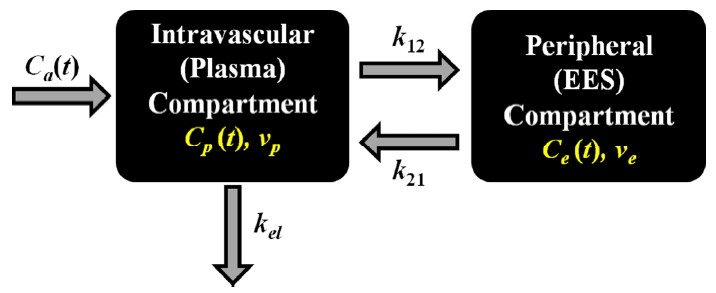
\includegraphics[width = 11cm]{img/diagram2}
	\caption{An example two compartment model \cite{khalifa2014models}.}
	\label{fig:diagram2}
\end{figure*}

The compartment PK models decribe complex blood-tissue exchanges and their theory is based on the differential mass balance equations \cite{sourbron2011tracer}. 
An example of the system decribed by two compartments is presented on Figure \ref{fig:diagram2}.


\subsubsection{Concentration time courses}
  

 



\begin{figure*}
	\centering
	\subfloat[Kidney time course]{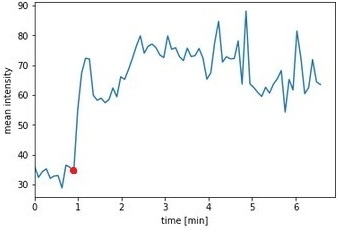
\includegraphics[width=6 cm]{img/timecourse_kidney}}\quad
	\subfloat[Aorta time course]{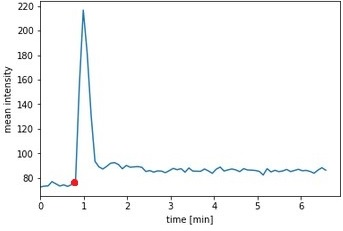
\includegraphics[width=6 cm]{img/timecourse_aorta}}\\		
\caption{Sample average time-courses for renal parenchyma (a) and aorta (b). The last point of baseline is marked with red dot.}
\label{fig:point}
\end{figure*}

Obtained time-concentration curves were then fitted to the described in the next sections PK models.





\subsubsection{GFR estimation}
Having calculated the $K_{trans}$ parameter the glomelural filtration rate can be computed according to the formula:
\begin{equation}
	\label{eq:gfr}
	GFR = K_{trans}V_{parenchyma}(1-H_{ct}) 
\end{equation}

\begin{figure*}
	\centering
	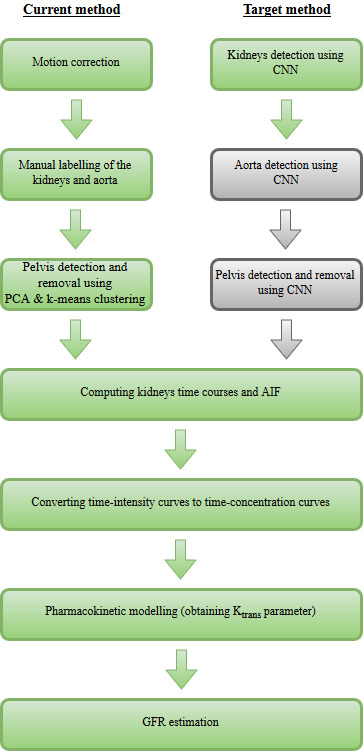
\includegraphics[height = 18cm]{img/methods}
	\caption{}
	\label{fig:methods}
\end{figure*}

\end{comment}
